\documentclass{article}
\usepackage[utf8]{inputenc}
\usepackage{amsmath}
\usepackage{float}
\usepackage{listings}
\usepackage[pdftex]{graphicx}
\usepackage{amssymb}
\usepackage{subcaption}
\usepackage{cancel}
%---------------------------------------------------------
\author{Pratik Aghor}
\title{HW $\# 1$: Basic Fluid Mechanics}
\date{\today}  % Toggle commenting to test

\begin{document}

\maketitle
%--------------------------------------------------------
\section{Q $1$: Constitutive Relationships}
%--------------------------------------------------------
Hypothesized:
\begin{itemize}
 \item The deviotric stress tensor $d_{ij}$ is only a function of gradients in velocities and not the velocities themselves (Galilean invariance): $d_{ij}\equiv d_{ij}(\frac{\partial u_{k}}{\partial x_{l}})$.
 \item Not just that, it is a linear function (details in the handout for the time-scales argument):
 $d_{ij} = A_{ijkl} \frac{\partial u_{k}}{\partial x_{l}}$.
 \item Isotropic: $A_{ijkl} = \mu \delta_{ik}\delta_{jl} + \mu' \delta_{il}\delta_{jk} + \mu'' \delta_{ij}\delta_{kl}$.
\end{itemize}
%---------------
\subsection*{(a): $\mu = \mu'$:}
%---------------
Since $\sigma_{ij}$ is symmetric, so is $d_{ij}$. 

\begin{align}\label{eq:dij_symm}
    \begin{split}
     d_{ij} &= (\mu \delta_{ik}\delta_{jl} + \mu' \delta_{il}\delta_{jk} + \mu'' \delta_{ij}\delta_{kl})\frac{\partial u_{k}}{\partial x_{l}} \\  
     d_{ji} &= (\mu \delta_{jk}\delta_{il} + \mu' \delta_{jl}\delta_{ik} + \mu'' \delta_{ij}\delta_{kl})\frac{\partial u_{k}}{\partial x_{l}} \\ 
     \because d_{ij} & = d_{ji} \Rightarrow d_{ij} - d_{ji} = 0\\
    & \Rightarrow \boxed{\mu = \mu'}.
    \end{split}
\end{align}

%---------------
\subsection*{(b): $A_{ijkl} = A_{ijlk}$:}
%---------------
$$A_{ijkl} = \mu (\delta_{ik}\delta_{jl} + \delta_{il}\delta_{jk}) + \mu'' \delta_{ij}\delta_{kl}$$

$$
A_{ijlk} = \mu (\delta_{il}\delta_{jk} + \delta_{ik}\delta_{jl}) + \mu'' \delta_{ij}\delta_{kl}
$$

By inspection, $A_{ijkl} = A_{ijlk}$. 

%---------------
\subsection*{(c)}
%---------------
Substituting $\frac{\partial u_{k}}{\partial x_{l}} = e_{kl} + r_{kl} = e_{kl} - \frac{1}{2} \varepsilon_{klm}\omega_{m}$, we have:

\begin{align}
 \begin{split}
  d_{ij} &= A_{ijkl} (e_{kl} - \frac{1}{2} \varepsilon_{klm}\omega_{m}) \\
  d_{ij} &= A_{ijlk}(e_{lk} - \frac{1}{2} \varepsilon_{lkm}\omega_{m}) \\
  \textrm{adding the two equations and noting: } \varepsilon_{klm} &= -\varepsilon_{lkm}, e_{kl} =e_{lk}, A_{ijkl} = A_{ijlk}  \\
  &\boxed{d_{ij} = A_{ijkl} e_{kl}}.
 \end{split}
\end{align}
%---------------
\subsection*{(d)}
%---------------
Finally, $d_{ii} = 0$, since by construction, $d_{ij}$ is deviotric.

\begin{align}
 \begin{split}
  d_{ii} & =[ \mu (\delta_{ik}\delta_{il} + \delta_{il}\delta_{ik}) + \mu'' \cancelto{3}{\delta_{ii}}\delta_{kl}] \frac{\partial u_{k}}{\partial x_{l}}\\
  0 &= 2 \mu \delta_{ik}\delta_{il} + 3 \mu'' \delta_{kl}\\
  & \textrm{contracting with} \delta_{kl} \\
  0 & =2 \mu \delta_{ik}\delta_{il}\delta_{kl} + 3 \mu'' \delta_{kl}\delta_{kl}\\
  0 &= 2 \mu \cancelto{\delta_{ll} = 3}{\delta_{il}\delta_{il}} + 3 \mu'' \cancelto{3}{\delta_{kk}}\\
  0 &= 2\mu + 3 \mu'' \\
  & \boxed{\mu'' = -\frac{2}{3} \mu}.
 \end{split}
\end{align}
%---------------
\subsection*{(e)}
%---------------
Putting it all together:
\begin{align}\label{eq:constitutive_relation}
 \begin{split}
  d_{ij} & = A_{ijkl} e_{kl},\\
  &= \mu \left(\delta_{il}\delta_{jk} + \delta_{ik}\delta_{jl} - \frac{2}{3}\delta_{ij}\delta_{kl} \right) e_{kl},\\
  & = 2\mu e_{ij} - \frac{2}{3} e_{kk} \delta_{ij},\\
  & = 2 \mu \left[e_{ij} - \frac{\Delta}{3} \delta_{ij} \right].  
 \end{split}
\end{align}
$\boxed{d_{ij} = 2 \mu \left[e_{ij} - \frac{\Delta}{3} \delta_{ij} \right]}$.

%-------------------------------------------------------
\section{Q $2$: Energy Equation:}
%-------------------------------------------------------
We want to apply the first law of thermodynamics to obtain the energy balance for a material volume of fluid.
%---------------
\subsection*{(a)}
%---------------
\begin{equation}\label{eq:first_law}
 de = \delta q + \delta w.
\end{equation}
Here
\begin{equation}
 e = \frac{1}{2}u_{i}u_{i} + \hat{u},
\end{equation}
where $e$ is the total energy (kinetic $+$ potential), $\hat{u}$ is the internal energy, $de$ is a small change in $e$ and  $\delta q, \delta w$ are infinitesimal heat added to and work done on the system. An alternative form of \ref{eq:first_law} is
\begin{equation}\label{eq:alternate_first_law}
 \frac{DE}{Dt} = \dot{Q} + \dot{W},
\end{equation}
where $E$ is the total energy of the material volume and $\dot{Q}$ and $\dot{W}$ represent the rates of energy transferred to the system as heat or work.   

To determine $\dot{Q}$, we assume that there are no heat sources or sinks and neglect radiative transfer. The only mode of heat transfer is conduction and we assume \textbf{Fourier's law} of heat conduction, which relates the heat flux per unit area per unit time ($\dot{q_{c}}_{i}$ with conductivity ($\kappa$, a material property) and the local temperature $T$. 
\begin{equation}\label{eq:Fourier_law}
 \dot{q_{c}}_{j} = - \kappa \frac{dT}{dx_{j}}.
\end{equation}

For a surface $S$, consider an infinitesimal surface $dS$. If the normal points out in the $n_{j}$ direction,
\begin{align}\label{eq:dotQ}
 \begin{split}
  \dot{Q} & = -\int_{S}\dot{q_{c}}_{j} n_{j} dS \\
  & = \int_{S}  \kappa \frac{\partial T}{\partial x_{j}} n_{j} dS \\
  & = \int_{V} \frac{\partial}{\partial x_{j}}\left( \kappa \frac{\partial T}{\partial x_{j}} \right) dV \textrm{ ...Gauss's divergence theorem}.
 \end{split}
\end{align}

The rate of work done involves surface and body (limited to gravity) forces:
\begin{align}\label{eq:dotW}
 \begin{split}
  \dot{W} & = \int_{S} \sigma_{ij} u_{i} n_{j} dS + \int_{V} \rho g_{i} u_{i} dV \\
 & = \int_{V} \bigg[\frac{\partial}{\partial x_{j}}(\sigma_{ij} u_{i}) + \rho g_{i} u_{i}\bigg] dV.
 \end{split}
\end{align}

Therefore, we obtain the equation for the total energy:
\begin{align} \label{eq:etotal}
 \begin{split}
    & \rho \int_{V} \frac{De}{Dt} dV =   \int_{V} \bigg[\frac{d}{d_{j}}\left( \kappa \frac{dT}{dx_{j}} \right) + \frac{\partial}{\partial x_{j}}(\sigma_{ij} u_{i}) + \rho g_{i} u_{i} \bigg] dV\\
    & \boxed{\rho \frac{de}{dt} = \frac{d}{d_{j}}\left( \kappa \frac{dT}{dx_{j}} \right) + \frac{\partial}{\partial x_{j}}(\sigma_{ij} u_{i}) + \rho g_{i} u_{i} } \textrm{ ... Since dV arbitrary.}
 \end{split}
\end{align}

%---------------
\subsection*{(b)}
%---------------

To obtain the equation for the kinetic energy of the fluid, we take a dot product of the Cauchy's equations of motion with $u_{i}$ and use the fact that $u_{i} \frac{Du_{i}}{Dt} = \frac{1}{2} \frac{D u_{i}u_{i}}{Dt}.$

\begin{align}\label{eq:ke}
 \begin{split}
    u_{i} \bigg [\rho \frac{Du_{i}}{Dt} &= \frac{\partial}{\partial x_{j}} \sigma_{ij} + \rho g_{i} \bigg]\\
    \rho\frac{1}{2}\frac{D u_{i}u_{i}}{Dt} & = u_{i}\frac{\partial}{\partial x_{j}} \sigma_{ij} + \rho g_{i} u_{i}.
 \end{split}
\end{align}

Subtracting Eqn.(\ref{eq:ke}) from Eqn.(\ref{eq:etotal}), we obtain the equation for the internal energy of a fluid element:

\begin{equation}\label{eq:internal_energy}
\boxed {\rho \frac{D\hat{u}}{Dt} =  \frac{\partial}{\partial x_{j}}\left( \kappa \frac{\partial T}{\partial x_{j}} \right) + \sigma_{ij} \frac{\partial u_{i}}{\partial x_{j}} }.
\end{equation}
%---------------
\subsection*{(c)}
%---------------
Writing $\frac{\partial u_{i}}{\partial x_{j}} = e_{ij} + r_{ij}$, where $e_{ij} = \frac{1}{2}\left[\frac{\partial u_{i}}{\partial x_{j}} + \frac{\partial u_{j}}{\partial x_{i}} \right]$ and $r_{ij} = \frac{1}{2}\left[\frac{\partial u_{i}}{\partial x_{j}} - \frac{\partial u_{j}}{\partial x_{i}} \right]$ are the symmetric strain rate tensor and the rotation tensor, respectively, we obtain:

\begin{align}\label{eq:simplify_stress_work}
 \begin{split}
  \sigma_{ij} \frac{\partial u_{i}}{\partial x_{j}} &= \sigma_{ij} (e_{ij} + r_{ij})\\
  & = \sigma_{ij} e_{ij}.
 \end{split}
\end{align}

The last term vanishes because $\sigma_{ij}$ is a symmetric tensor and its dot contraction with an anti-symmetric $r_{ij}$ will be identically zero.

Substituting Eqn.(\ref{eq:simplify_stress_work}) into the internal energy equation, Eqn. (\ref{eq:internal_energy}) and substituting the expression for the stress tensor,

\begin{align}\label{eq:internal_energy_2}
 \rho \frac{D\hat{u}}{Dt} &=\frac{\partial}{\partial x_{j}}\left( \kappa \frac{\partial T}{\partial x_{j}} \right) + \sigma_{ij} e_{ij} \\
 & = \frac{\partial}{\partial x_{j}}\left( \kappa \frac{\partial T}{\partial x_{j}} \right) + \left[ -p_{t} \delta_{ij} + 2 \mu \left(e_{ij} - \frac{1}{3} \Delta \delta_{ij} \right) \right]e_{ij}\\
 &= \frac{\partial}{\partial x_{j}}\left( \kappa \frac{\partial T}{\partial x_{j}} \right) + -p_{t} \Delta + 2\mu \left(e_{ij}e_{ij} - \frac{1}{3}\Delta^{2} \right)
\end{align}
%---------------
\subsection*{(d): Writing the internal energy equation in terms of directly measurable quantities using the $2^{nd}$ law of thermodynamics:}
%---------------
The Gibbs equation is another way of writing the first law of thermodynamics:
\begin{equation}\label{eq:gibbs}
 Tds = d\hat{u} + p_{t} dv
\end{equation}

Here, the specific entropy $s \equiv s(\hat{u}, v) $ and the goal is to transform it to $s \equiv s(T, p_{t})$, where $T$ and $p_{t}$ are temperature and thermodynamic pressure, respectively.

We start by introducing the Gibbs potential $g = \hat{u} + p_{t}v - Ts$. This immediately implies the following:
\begin{align}
 \begin{split}
  & dg = \cancel{d\hat{u}} + \cancel{p_{t}dv} + vdp_{t} - \cancel{Tds} - sdT \\
  & dg = vdp_{t} - sdT. \\
  & \Rightarrow \frac{\partial g}{\partial p_{t}}\bigg|_{T} = v, \frac{\partial g}{\partial T}\bigg|_{p_{t}} = -s
 \end{split}
\end{align}

Now, considering $\frac{\partial^{2}g}{\partial p_{t} \partial T} = \frac{\partial^{2}g}{\partial T \partial p_{t}}$

\begin{align}\label{eq:maxwell_relation}
 \begin{split}
  \frac{\partial v}{\partial T}\bigg|_{p_{t}} = - \frac{\partial s}{\partial p}\bigg|_{T} 
 \end{split}
\end{align}
gives the required Maxwell relation.

Now, since we want $s \equiv s(T, p_{t})$,
\begin{align}
 \begin{split}
  ds &= \frac{\partial s}{\partial T}\bigg|_{p_{t}} dT+ \frac{\partial s}{\partial p_{t}}\bigg|_{T} dp_{t}\\
  T ds &= T\frac{\partial s}{\partial T}\bigg|_{p_{t}} dT+ T\frac{\partial s}{\partial p_{t}}\bigg|_{T} dp_{t}\\
  T ds &= c_{p} dT - T  \frac{\partial v}{\partial T}\bigg|_{p_{t}} dp_{t}\\
  Tds &= c_{p} dT - (\beta v T)dp_{t}
 \end{split}
\end{align}
where $c_{p} = T\frac{\partial s}{\partial T}\bigg|_{p_{t}}$ is the specific heat capacity at constant pressure and $\beta = \frac{1}{v}\frac{\partial v}{\partial T}\bigg|_{p_{t}} dp_{t}$ is the coefficient of thermal expansion.

Finally, writing $v = 1/\rho$, we obtain the material derivative for entropy.

\begin{align}\label{eq:entropy}
 \begin{split}
  T \frac{Ds}{Dt} &= c_{p} \frac{DT}{Dt} - \frac{\beta T}{\rho}\frac{Dp_{t}}{Dt}\\
  & = \frac{D\hat{u}}{Dt} - \frac{p_{t}}{\rho^{2}}\frac{D\rho}{Dt}\\
  & = \frac{\lambda \Delta^{2}}{\rho} + \Phi + \frac{1}{\rho} \frac{\partial }{\partial x_{j}}\left(\kappa \frac{\partial T}{\partial x_{j}} \right).
 \end{split}
\end{align}
%---------------
\subsection*{(e):}
%---------------
Assuming that bulk viscous effects are negligible $\lambda = 0 $ and $p_{t} = p$, i.e., thermodynamic and mechanical pressures are equal.This yields the equation for the evolution of temperature. 

\begin{equation}\label{eq:temperature}
 c_{p}\frac{DT}{Dt} = \frac{\beta T}{\rho}\frac{Dp}{Dt} + \Phi + \frac{1}{\rho}\nabla.(\kappa \nabla T),
\end{equation}
which must be supplemented by an equation of state $p \equiv p(\rho, T)$ in order to close the system. 

%-------------------------------------------------------
\section{Q $3$: $\tau_{i} = \sigma_{ij} n_{j}$}
%-------------------------------------------------------
Here, I am basically reproducing the calculation in $\S 1.3$ from \cite{batchelor2000introduction}. We consider a tetrahedron $OABC$ as shown in the Fig. such that $A(AOC) = \delta A_{2}, A(AOB)=\delta A_{3}. A(BOC) = \delta A_{1}$ and $A(ABC) = \delta A$, with the normals, $-\underline{a}, -\underline{b}, -\underline{c}$ and $\underline{n}$ respectively. Since this is an infinitesimal tetrahedron, we drop the dependence of $\Sigma$ on $\underline{x}, t$, i.e., $ \underline{\Sigma} (\underline{x}, t, \underline{n}) \equiv \underline{\Sigma} (\underline{n})$. 
\begin{figure}[H]
    \centering
    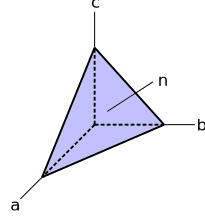
\includegraphics[scale = 0.2]{Figs/tetrahedron.png}
    \caption{An infinitesimal tetrahedron}
    \label{fig:tetrahedron}
\end{figure}

At the leading order, surface forces ($O(\delta l^{2})$) dominate the body forces ($O(\delta l^{3})$) since $\delta l \ll 1$. Therefore, the force balance gives:

\begin{align}\label{eq:tetrahedron_sf_balance}
\begin{split}
 & \underline{\Sigma}(\underline{n})\delta A + \underline{\Sigma}(-\underline{a})\delta A_{1} + \underline{\Sigma}(-\underline{b})\delta A_{2} + 
 \underline{\Sigma}(-\underline{c})\delta A_{3} = 0,\\
 & \underline{\Sigma}(\underline{n})\delta A - \underline{\Sigma}(\underline{a})\delta A_{1} - \underline{\Sigma}(\underline{b})\delta A_{2} - 
 \underline{\Sigma}(\underline{c})\delta A_{3} = 0,\\
 & \underline{\Sigma}(\underline{n})\delta A = \underline{\Sigma}(\underline{a})\delta A_{1} + \underline{\Sigma}(\underline{b})\delta A_{2} + 
 \underline{\Sigma}(\underline{c})\delta A_{3}.
\end{split}
\end{align}

We know that the volume of a tetrahedron is given by 
\begin{align}\label{eq:tetrahedron_vol}
 \begin{split}
  dV &= \frac{1}{6}\underline{a} \cdot \left(\underline{b} \times \underline{c} \right)\\
  &= \frac{1}{6} (\perp \textrm{distance})(\textrm{area of the suface})
 \end{split}
\end{align}

Since it is the same tetrahedron, we can express the above formula in $4$ different ways, one corresponding to each surface, and all of them must yield the same result. For example $\delta A_{1} \cdot \underline{a} = \delta A \cdot \underline{n}$, giving $\delta A_{1} = \delta A (\underline{a}\cdot \underline{n})$. 
Cancelling factors of $1/6$, we obtain:  

\begin{align}\label{eq:area_relations}
\begin{split}
 \delta A_{1} &= \delta A (\underline{a} \cdot \underline{n}), \\
 \delta A_{2} &= \delta A (\underline{b} \cdot \underline{n}), \\
 \delta A_{3} &= \delta A (\underline{c} \cdot \underline{n}), \\
\end{split}
\end{align}

Substituting Eqn.(\ref{eq:area_relations}) into Eqn. (\ref{eq:tetrahedron_sf_balance}), we obtain
\begin{align}
 \begin{split}
  \underline{\Sigma}(\underline{n}) &= \left[\underline{\Sigma}(\underline{a}) \underline{a} + \underline{\Sigma}(\underline{b}) \underline{b} + \underline{\Sigma}(\underline{c}) \underline{c}\right]\cdot \underline{n} \\
  \Sigma_{i}(\underline{n}) &= \left[\Sigma_{i}(\underline{a}) a_{j} + \Sigma_{i}(\underline{b}) b_{j} + \Sigma_{i}(\underline{c}) c_{j}\right]n_{j}\\
 \end{split}
\end{align}
The quantity in the brackets on the RHS is a generalization of a second order tensor. Hence, $\boxed{\tau_{i}(\underline{n}) = \Sigma_{i}(\underline{n}) = \sigma_{ij} n_{j}}.$ QED.
%------------------------------------------------------
\section{Q $4$: Level Sets of Stream Function $\psi$:}
%------------------------------------------------------
%---------------
\subsection*{(a)}
%---------------

First, we start by deriving an equation for a streamline. Streamline is defined as a line everywhere parallel to the velocity field. If $d\underline{s} = dx_{i}\underline{e_{i}}$ is the arclength along the streamline, we must have $d\underline{s} \times \underline{u} = 0$. 
\begin{align}\label{eq:streamline}
 \begin{split}
    (d\underline{s} \times \underline{u})_{k} &= \varepsilon_{ijk} dx_{i} u_{j} \\
    \underline{0} & = \varepsilon_{ijk} dx_{i} u_{j}\\
    \underline{0} &= (w \, dy -  v \, dz )e_{1} + (w \, dx  - u \, dz )e_{2} +(v\,dx - u \, dy)e_{3}
 \end{split}
\end{align}

In $2D$, we have $v\,dx - u \, dy = 0$ or $dy/dx = v/u$ to be the equation of a streamline. 

Now, let $\psi$ be a stream function in $2D$, such that $\frac{\partial \psi}{\partial x} = - v$ and $\frac{\partial \psi}{\partial y} = u$. Differentiating, we obtain:
\begin{align}\label{eq:psi_diff}
 \begin{split}
  d\psi & = \frac{\partial \psi}{\partial x} dx + \frac{\partial \psi}{\partial y} dy, \\
  & = -v \, dx + u \, dy. 
 \end{split}
\end{align}

For a $\psi = constant$ surface, we have $d\psi = 0$, yielding $-v \, dx + u \, dy = 0$ or $dy/dx = v/u$, which is an equation of a streamline as derived above. Hence, the level sets of a stream function are the streamlines. QED. 
%---------------
\subsection*{(b)}
%---------------

Now, we consider two different streamlines with different values of $\psi$, say $\psi = \psi_{1}$ on one streamline and $\psi = \psi_{2}$ on the other. 

\begin{figure}[H]
    \centering
    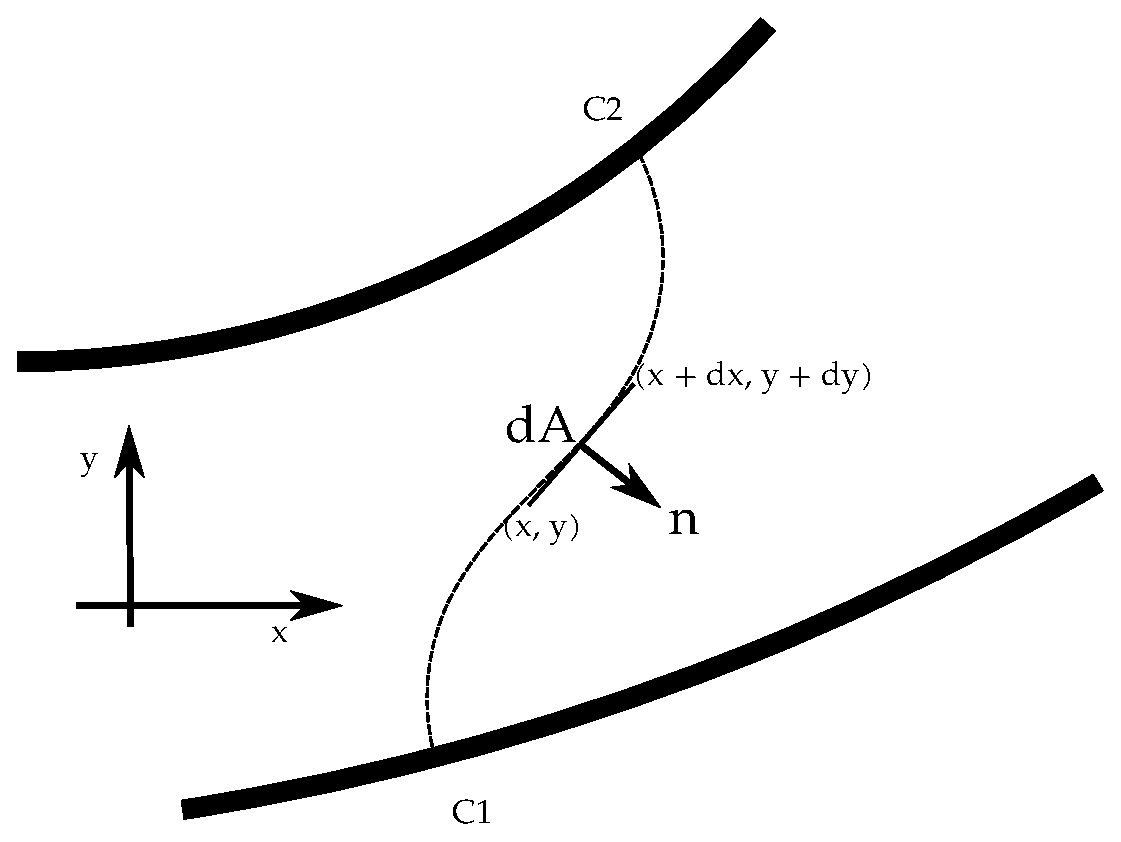
\includegraphics[scale = 0.4]{Figs/across_streamlines.eps}
    \caption{}
    \label{fig:across_streamlines}
\end{figure}
Let $C_{1}C_{2}$ be a curve spanning $\psi=\psi_{1}$ and $\psi=\psi_{2}$. Let $dA$ be the infinitesimal area per unit depth ($b$) on this curve. 

By construction, $\hat{n} \perp d\underline{A}$. Since $d\underline{A} \parallel (dx \, \hat{i} + dy \, \hat{j})$, we have $\hat{n} dA = dy \, \hat{i} - dx \, \hat{j}$. 
The volume flow rate per unit depth ($b$) across $C_{1}C_{2}$ is given by 

\begin{align}
 \begin{split}
  Q = \dot{m}/\rho &= \int_{C_{1}}^{C_{2}} \underline{u}\cdot \underline{n} dA \\
  &= \int_{C_{1}}^{C_{2}} \underline{u}\cdot (dy \, \hat{i} - dx \, \hat{j}) \\
  &= \int_{C_{1}}^{C_{2}}(u \, dy - v\, dx) \\
  &= \int_{C_{1}}^{C_{2}} d\psi \\
  &= \psi_{2} - \psi_{1}.
 \end{split}
\end{align}
Hence the volume flow rate per unit depth across level surfaces of $\psi$ is given by the difference between the values of $\psi$ on the two level surfaces. QED.
%------------------------------------------------------
\section{Q $5$: Decomposing Shear Flow: $\underline{u}=\beta y \underline{e}_{x}$}
%------------------------------------------------------
We will work in only $2D$ - $x-y$ plane. For this velocity field, the writing decomposing the velocity gradient tensor ($\nabla \underline{u}$) into symmetric ($e_{ij}$) and anti-symmetric($r_{ij}$) parts in the matrix form:

\begin{equation}\label{eq:gradu_decomp}
 \begin{bmatrix}
  0 & \beta \\
  0 & 0
 \end{bmatrix}
= \begin{bmatrix}
  0 & \beta/2 \\
  \beta/2 & 0
 \end{bmatrix}
 + \begin{bmatrix}
  0 & \beta/2 \\
  -\beta/2 & 0
 \end{bmatrix}.
\end{equation}

Let us focus on the symmetric part $e_{ij}$. Since $e_{ij}$ is symmetric, it has real eigenvalues and it is diagonalizable. 

Finding eigenvalues of $e_{ij}$:
\begin{align}\label{eq:eij_eig}
 \begin{split}
  \textrm{det}|e_{ij} - \lambda \delta_{ij}| &= 0\\
  \lambda^{2} - \beta^{2}/4 &= 0\\
  \lambda_{1, 2} &= \pm \beta/2.
\end{split}
\end{align}

The corresponding eigenvectors can be easily calculated $v_{1} = [1/\sqrt{2},1/\sqrt{2}]$ corresponding to $\lambda_{1} = \beta/2$ and $v_{2} = [1/\sqrt{2},-1/\sqrt{2}]$ corresponding to $\lambda_{2} = -\beta/2$. In the co-ordinate system of $(v_{1}, v_{2})$, $e_{ij}$ will only have normal components as the eigenvalues. 

In other words if $V = [v_{1} | v_{2}]$,i.e., if $V = \begin{bmatrix}
  1/\sqrt{2} & 1/\sqrt{2} \\
  1/\sqrt{2} & -1/\sqrt{2}                                                         \end{bmatrix}
$, then 

\begin{equation}
 V^{-1}e V = \begin{bmatrix}
              \beta/2 & 0\\
              0 & -\beta/2
             \end{bmatrix}.
\end{equation}
This constitues the pure straining components shown with the red arrows in Fig. \ref{fig:shearflow_decomp}. 

To find out the rotation, we use the relation $\omega_{i} = \varepsilon_{ijk} r_{kj} = - \varepsilon_{ijk} r_{jk}$.
This immediately gives $\omega_{3} = -\beta$, giving the sense of rotation of the flow, which will be clockwise, as indicated by the blue arrows in Fig. \ref{fig:shearflow_decomp}. The superposition of the two flows recovers back the simple shear flow velocity profile. 
\begin{figure}[H]
    \centering
    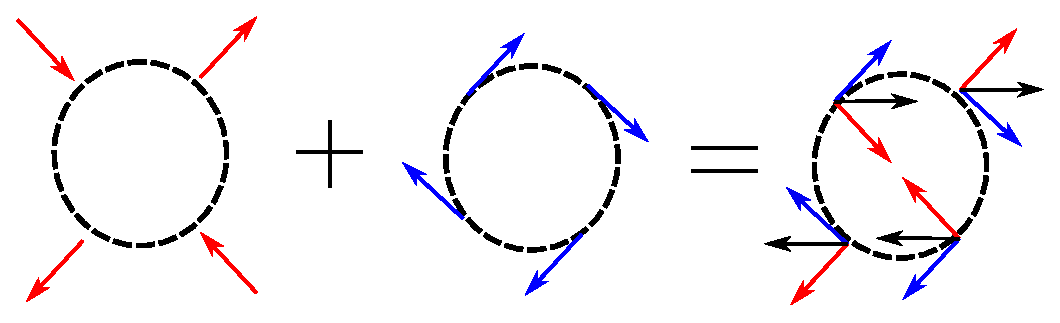
\includegraphics[scale = 0.8]{Figs/shearflow_decomp.eps}
    \caption{Superposition of pure straining (red) and rotation (blue) yields the simple shear flow.}
    \label{fig:shearflow_decomp}
\end{figure}
%------------------------------------------------------
\section{Q $6$: Stagnation-point Flow in Eulerian and Lagrangian Coordinates:}
%------------------------------------------------------
Planar stagnation point flow Eulerian representation $\underline{u} = \alpha x \underline{e}_{x} - \alpha y \underline{e}_{y}$ for some constant $\alpha > 0$.
%---------------
\subsection*{(a) Stream function:} 
%---------------
Computing the divergence of the flow $\nabla\cdot \underline{u} = \alpha - \alpha = 0$. The flow is also $2D$. Hence a stream function will exist for this flow. 

\textbf{Calculating the stream function $\psi$:}
$\psi$ must satisfy: $\frac{\partial \psi}{\partial x} = - \alpha y, \frac{\partial \psi}{\partial y} = -(\alpha x) = - \alpha x$. 

Integrating the $x$-equation, we obtain
$\psi(x, y) = \alpha xy + g(y)$ for some unknown $g(y)$. Substituting this into the $y$-equation gives

\begin{align}
 \begin{split}
 & \alpha x + g'(y) = \alpha x, \\
 & \Rightarrow g(y) = c,\\
 & \Rightarrow \psi(x, y) = \alpha xy + c,
 \end{split}
\end{align}

where $c$ is some arbitrary constant, which we set to $0$ without loss of generality, since the physically important fields such as velocities, depend on the gradients of $\psi$ and not $\psi$ itself. Therefore,
$\boxed{\psi(x, y) =  \alpha xy}$.
%---------------
\subsection*{(b) Incompressible and Irrotational:}
%---------------
\begin{enumerate}
 \item Incompressible - proved in above subsection $\nabla \cdot \underline{u} = 0$. 
 \item Irrotational?: Calculating vorticity $\nabla \times \underline{u} = \left(\frac{\partial v}{\partial x} - \frac{\partial u}{\partial y} \right)\underline{e}_{z} = \underline{0}$. Hence the flow is irrotational.
\end{enumerate}
%---------------
\subsection*{(c) Material derivative of pollutant concentration:}
%---------------
Given: $c(x, y, t) = \beta x^{2}y e^{-\alpha t}$. Rate of change of pollutant concentration of a fluid parcel over time 
\begin{align}\label{eq:pollutant_concentration}
 \begin{split}
  \frac{Dc}{Dt} & = \frac{\partial c}{\partial t} + u \frac{\partial c}{\partial x} + v \frac{\partial c}{\partial y} \\
  &= e^{-\alpha t}\left[\beta x^{2}y(-\alpha) + \alpha x \cdot 2 \beta x y - \alpha y \cdot \beta x^{2}\right]\\
  & = 0.
  \end{split}
\end{align}
Hence the concentration of pollutant for a given fluid parcel remains constant (does not change) over time. 
%---------------
\subsection*{(d) Path lines:}
%---------------
The equation of the path lines will be given by
\begin{align}\label{eq:pathlines}
 \begin{split}
  \frac{dx}{dt} &= \alpha x \\
  \frac{dy}{dt} &= -\alpha y.
 \end{split}
\end{align}
%---------------
\subsection*{(e) Lagrangian representation:}
%---------------
We define $\underline{X}(\underline{x}_{0}, t)$ to be the Lagrangian co-ordinate of a fluid particle that was at $\underline{x}_{0}$ at $t = 0$. At time $t=t$, let the particle be at $(x,y)$, the velocity of the particle at that instant must match the Eulerian velocity $\underline{u}(x, y)$ at that spatial location. Therefore, we must have,
\begin{align}\label{eq:lagrangian_coord}
 \begin{split}
  \frac{\partial X}{dt}\bigg|_{\underline{x}_{0}} &= \alpha X \Rightarrow X = x_{0} e^{\alpha t} \\
  \frac{\partial Y}{dt}\bigg|_{\underline{x}_{0}} &= -\alpha Y \Rightarrow Y = y_{0} e^{-\alpha t} \\
  \end{split}
\end{align}

We have calculated the above derivatives at a spatial point $(x, y)$ or in the Lagrangian terms, when the particle is at $(X, Y)$. We also stress that this is done for a \textbf{fixed} $(x_{0}, y_{0})$, meaning we are talking about a specific fluid parcel that was at $(x_{0}, y_{0})$ at $t=0$ and now (at $t=t$) is at $(X, Y)$. 
TO obtain the Lagrangian velocity $\underline{U}(X, Y, t)$ at $(X, Y)$, we must differentiate $(X(x_{0}, y_{0}, t),Y(x_{0}, y_{0}, t))$ twice with respect to (w.r.t.) time. 

\begin{align}\label{eq:lagrangian_velo}
 \begin{split}
  U & = \frac{\partial X}{dt}\bigg|_{\underline{x}_{0}} = \alpha x_{0} e^{\alpha t} \\
  V &= \frac{\partial Y}{dt}\bigg|_{\underline{x}_{0}} = -\alpha y_{0} e^{-\alpha t}
 \end{split}
\end{align}
Hence $\boxed{\underline{U}(X, Y, t) = (\alpha x_{0} e^{\alpha t}, -\alpha y_{0} e^{-\alpha t})}$.

This immediately implies
\begin{align}\label{eq:lagrangian_acc}
 \begin{split}
  \frac{\partial U}{dt}\bigg|_{\underline{x}_{0}} & = \alpha^{2} x_{0} e^{\alpha t} = \alpha^{2}X \\
  \frac{\partial V}{dt}\bigg|_{\underline{x}_{0}} &= \alpha^{2} y_{0} e^{-\alpha t} = \alpha^{2}Y
 \end{split}
\end{align}
in terms of $(X, Y)$, 
$\boxed{\frac{\partial \underline{U}}{\partial t} \bigg|_{\textrm{at} (X, Y)} = (\alpha^{2}X, \alpha^{2}Y)}$.

On the other hand, we can find the material derivative of the Eulerian velocity as follows:
\begin{align}\label{eq:eulerian_acc}
 \begin{split}
   \frac{Du}{Dt} &= \cancelto{0}{\frac{\partial u}{\partial t}} + u\frac{\partial u}{\partial x} + v \cancelto{0}{\frac{\partial u}{\partial y}},\\
   \frac{Du}{Dt} & = \alpha^{2}x \\
   \frac{Dv}{Dt} &= \cancelto{0}{\frac{\partial v}{\partial t}} + u \cancelto{0}{\frac{\partial v}{\partial x}} + v\frac{\partial v}{\partial y} ,\\
   \frac{Dv}{Dt} & = \alpha^{2}y \\
 \end{split}
\end{align}
Comparing at $(X,Y) = (x, y)$, we obtain $\boxed{\frac{\partial \underline{U}}{\partial t} \big|_{(X, Y)} = \frac{D\underline{u}}{Dt}}$.

For the concentration of the pollutant, the expression in part (c) is an Eulerian expression, in that it gives the concentration as a function of $(x, y, t)$. If, however, we are following the same fluid particle which was at $\underline{x}_{0}$ at $t = 0$ and is now at $(X, Y)$, we can write a Lagrangian version for that fluid parcel at the point $(X, Y)$.
\begin{align}\label{eq:lagrangian_conc}
 \begin{split}
  C(X, Y, t) &= \beta X^{2}Ye^{-\alpha t}\\
  &= \beta x_{0}^{2} \cancel{e^{2\alpha t}}\cdot y_{0} \cancel{e^{-\alpha t}} \cdot \cancel{e^{-\alpha t}}\\
  &= \beta x_{0}^{2}y_{0}.
 \end{split}
\end{align}
This immediately implies that $\frac{\partial C}{\partial t}\big|_{X, Y} = 0$, confirming that the concentration of a particular blob of fluid does not change with time!
%------------------------------------------------------
\section{Q $7$: Free Surface of a Rotation Bucket of Water:}
%------------------------------------------------------
%---------------
\subsection*{(a) Failure of the Bernoulli Argument:}
%---------------
The Bernoulli argument fails because although the flow is inviscid, it is not irrotational. Hence expecting the value of $C$ to be the same across streamlines will lead to erroneous conclusions. 

%---------------
\subsection*{(b) Correct pressure distribution from Euler's Equations:}
%---------------
The velocity field is given by $\underline{u}= -\Omega  y \hat{e}_{x} + \Omega  x \hat{e}_{y} + 0 \hat{e}_{z}$.Writing Euler's equations in $x$ and $y$ directions:

\begin{align}\label{eq:euler_eqns}
 \begin{split}
  \rho \frac{Du}{Dt} &= -\frac{\partial p}{\partial x} \\
  \rho \frac{Dv}{Dt} &= -\frac{\partial p}{\partial y}\\
  \rho \frac{Dw}{Dt} &= -\frac{\partial p}{\partial z} + \rho g
 \end{split}
\end{align}

In the context of the given velocity field, Euler's equations take the following form:
\begin{align}\label{eq:bucket_euler_eqns}
 \begin{split}
  -\rho \Omega^{2} x &= -\frac{\partial p}{\partial x} \\
  -\rho \Omega^{2} y  &= -\frac{\partial p}{\partial y}\\
  0 &= -\frac{\partial p}{\partial z} + \rho g
 \end{split}
\end{align}

Integrating the $x$ equation, we obtain
$p(x, y, z) = \rho \Omega^{2} x^{2}/2 + f(y, z)$. Substituting this into the $y$ equation, we get:

$\frac{\partial f}{\partial y} = \rho \Omega^{2} y$, giving, $f(y, z) = \rho \Omega^{2} y^{2}/2 + h(z)$, so $p(x, y, z) = \rho \Omega^{2} (x^{2} + y^{2})/2 + h(z)$. 
Finally, substituting this into the $z$ equation, we obtain:
$p(x, y, z) = \rho \Omega^{2} (x^{2} + y^{2})/2 + \rho g z + c$ We set $c = 0$ without loss of generality. 

$\boxed{p(x, y, z) = \rho \Omega^{2} (x^{2} + y^{2})/2 + \rho g z}$. Hence, contours of constant pressure are paraboloids. 
%------------------------------------------------------
\section{Q $8$: Rayleigh Flat Plate Problem with Oscillating Boundary:}
%------------------------------------------------------
We consider a semi-infinite fluid lying above a plane
solid boundary at $y = 0$ and initially at rest. At time $t = 0$, the boundary begins to oscillate
periodically in its plane ($x$ direction) with $U(t) = U_{0} \sin{\Omega t}$.

We look for a unidirectional flow assuming:
\begin{align}\label{eq:Rayleigh_flat_plate_ansatz}
 \begin{split}
  & \boldsymbol{u} = u(y, t) \boldsymbol{e_{x}} \textrm{, where}\\
  & u(y, t) = U_{0} f(y) \sin{\Omega t} + U_{0} g(y) \cos{\Omega t}.
 \end{split}
\end{align}
The Navier-Stokes equations reduce to the diffusion equation:

\begin{equation}\label{eq:diffusion}
 \frac{\partial u}{\partial t} = \nu \frac{\partial^{2} u}{\partial t^{2}}.
\end{equation}

We solve the problem, noting that the governing equation is linear and real. Define $U(y, t)$ to be some complex velocity field. Express the boundary condition for $U$ as $U(0, t) = U_{0} \exp{i\Omega t}$. Assume $U(y, t) = U_{0} h(y) \exp{i\Omega t}$, then the BC at $y=0$ gives $h(0) = 1$. 

The the solution to the problem will be given by $u(y, t) = \textrm{Im}(U(y, t))$. Substituting $U(y, t) = U_{0} h(y) \exp{i\Omega t}$ in Eqn.(\ref{eq:diffusion}):

\begin{align}\label{eq:substituting_ansatz}
 \begin{split}
  U_{t} &= \nu U_{yy} \\
  i \Omega h &= \nu h_{yy}\\
  h_{yy} &- \frac{i\Omega}{\nu} h = 0\\
  h(y)  &= A \exp{\left(\sqrt\frac{i\Omega}{\nu}\right)y} + B \exp{\left(\sqrt\frac{-i\Omega}{\nu}\right)y}\\
  \because \sqrt{i} &= [\exp{(i\pi/2)}]^{1/2} = \exp{(i\pi/4)} =  \frac{1 + i}{\sqrt{2}}\\
  & = A \exp{\left(\frac{1 + i}{\sqrt{2}} \sqrt\frac{\Omega}{\nu}  y \right)} + B \exp{\left(-\frac{1 + i}{\sqrt{2}} \sqrt\frac{\Omega}{\nu}  y \right)}\\
  \because h(0) &= 1, h(\infty) = 0, \\
  h(y) &= \exp{\left(-\frac{1 + i}{\sqrt{2}} \sqrt\frac{\Omega}{\nu}  y \right)}.
 \end{split}
\end{align}

Therefore,
\begin{align}\label{eq:flat_plate_soln}
 \begin{split}
  U(y, t) &= U_{0} \exp{\left(-\frac{1 + i}{\sqrt{2}} \sqrt\frac{\Omega}{\nu}  y \right)} \exp{i\Omega t}\\
  &= U_{0} \exp{\left(- \sqrt\frac{\Omega}{2\nu}  y \right)} \exp{\left[i\left(-\sqrt\frac{\Omega}{2\nu}  y  + \Omega t\right)\right]}\\
  u(y, t) &=  U_{0} \exp{\left(- \sqrt\frac{\Omega}{2\nu}  y \right)} \sin{\left(- \sqrt\frac{\Omega}{2\nu}  y  + \Omega t\right)}.
 \end{split}
\end{align}

I wrote a small python code to plot the solution at different instances during one oscillation of the plate. 

\begin{figure}[H]
    \centering
    \includegraphics[scale = 0.8]{Figs/u_vs_y_diff_t.png}
    \caption{$T= \frac{2 \pi}{\Omega}$. Sample velocity profiles for $8$ different instances of time, for $\Omega = 1$, $\nu = 1$, $U_{0} = 0.1$.}
    \label{fig:oscillating_plate_soln}
\end{figure}

We can calculate the vorticity as follows:
\begin{align}
 \begin{split}
  \omega_{z} & = \cancelto{0}{\frac{\partial v}{\partial x}}-\frac{du}{dy} \\
  \omega_{z} &= U_{0}\left( \sqrt\frac{\Omega}{2\nu}  \right) \exp{\left(- \sqrt\frac{\Omega}{2\nu}  y \right)} \left[ \sin{\left(- \sqrt\frac{\Omega}{2\nu}  y  + \Omega t\right)} + \cos{\left(- \sqrt\frac{\Omega}{2\nu}  y  + \Omega t\right)}\right]
  \end{split}
\end{align}
So for all times, since the damping factor $\exp{\left(- \sqrt\frac{\Omega}{2\nu}  y \right)}$ is independent of time, the vorticity is constrained to a region of $y \sim O\left( \sqrt\frac{2\nu}{\Omega}\right)$.
%------------------------------------------------------
\section{Q $9$: Gravity Driven Film Flow:}
%------------------------------------------------------
%---------------
\subsection*{(a) BCs:}
%---------------
\begin{enumerate}
 \item \textbf{No slip} at $y = 0 \Rightarrow u(x, y=0, t) = 0$.
 %%
 \item \textbf{No normal-flow} at $y = 0 \Rightarrow v(x, y=0, t) = 0$.
 %%
 \item \textbf{Kinematic BC:} Consider a material parcel of fluid at the liquid-air interface. Represent the interface by $\mathcal{F}(x, y, t) \equiv y - h(x, t) = 0$. Since the material parcel moves along $mathcal{F} = 0$ surface, we have
 \begin{align}\label{eq:kinematic_bc}
  \begin{split}
   \frac{D\mathcal{F}}{Dt} & = \frac{\partial \mathcal{F}}{\partial t} + u\frac{\partial \mathcal{F} }{\partial x} + v\frac{\partial \mathcal{F} }{\partial y} \\
   0 &= \cancelto{-1}{\frac{\partial \mathcal{F} }{\partial h}} \frac{\partial h}{\partial t} + u \cancelto{-1}{\frac{\partial \mathcal{F} }{\partial h}} \frac{\partial h}{\partial x} + v \cancelto{1}{\frac{\partial \mathcal{F} }{\partial y}} \\
   v (x, h, t) &= \frac{\partial h}{\partial t} + u \frac{\partial h}{\partial x}.
  \end{split}
 \end{align}
 This holds for both right below and above the surface, yielding $2$ kinematic bcs.
 \begin{align}\label{eq:kinematic_bcs}
 \begin{split}
  v_{a}\bigg|_{(x, h, t)} &= \frac{\partial h}{\partial t} + u_{a}|_{(x, h, t)} \frac{\partial h}{\partial x} \\
  v_{l}\bigg|_{(x, h, t)} &= \frac{\partial h}{\partial t} + u_{l}|_{(x, h, t)} \frac{\partial h}{\partial x} \\
 \end{split}
 \end{align}
Another kinematic boundary condition that we require (because we are modeling air as a viscous fluid) is the continuity of the tangential velocity. 
\begin{equation}\label{eq:third_kinematic_bc}
 \underline{u_{l}}\cdot \hat{t}\big|_{y = h^{-}} = \underline{u_{a}}\cdot \hat{t}\big|_{y = h^{+}}
\end{equation}

%%
\item \textbf{Dynamic BC:} We neglect surface tension. First, we derive the expressions for the normal ($\hat{n}$ ) and tangent ($\hat t$) vectors at the surface. Since the surface is given by $\mathcal{F} = 0$, the normal will be parallel to $\nabla \mathcal{F}$, i.e.,  
\begin{align}\label{eq:nHat}
 \begin{split}
  \hat{n} &\parallel \left[\frac{\partial \mathcal{F}}{\partial x}, \frac{\partial \mathcal{F}}{\partial y} \right]\\
  & \parallel \left[-\frac{\partial h}{\partial x}, 1 \right]\\
  \hat{n} &= \frac{-\partial h/\partial x}{\sqrt{\left( \partial h/\partial x\right)^{2} + 1} } \hat{e}_{x} + \frac{1}{\sqrt{\left( \partial h/\partial x\right)^{2} + 1} } \hat{e}_{y}.
 \end{split}
\end{align}
To construct the unit tangent vector $\hat{t}$, we parametrize the surface $\mathcal{F}$ by $[x, h(x, t)]$. Then $\hat{t}\parallel \left[1, \frac{\partial h}{\partial x} \right]$. Also, the tangent vector will be perpendicular to $\hat{n}$. Normalizing:
\begin{equation}\label{eq:tHat}
 \hat{t} = \frac{1}{\sqrt{\left( \partial h/\partial x\right)^{2} + 1} } \hat{e}_{x} + \frac{\partial h/\partial x}{\sqrt{\left( \partial h/\partial x\right)^{2} + 1} } \hat{e}_{y}.
\end{equation}
Writing the stress balance in the normal direction
\begin{align}\label{eq:dynamic_bc_n}
 \begin{split}
  & n_{i}(\sigma_{l_{ij}} n_{j}) = n_{i}(\sigma_{a_{ij}} n_{j})\\
  & n_{1} \sigma_{l_{11}} n_{1} + n_{1} \sigma_{l_{12}} n_{2} + n_{2} \sigma_{l_{21}} n_{1} + n_{2} \sigma_{l_{22}} n_{2} =  n_{1} \sigma_{a_{11}}n_{1} + n_{1} \sigma_{a_{12}} n_{2} + n_{2} \sigma_{a_{21}} n_{1} + n_{2} \sigma_{a_{22}} n_{2} \\
  & \sigma_{l_{11}}(\partial h/ \partial x)^{2} + 2 \sigma_{l_{12}}(-\partial h/ \partial x) - \sigma_{l_{22}} = \sigma_{a_{11}}(\partial h/ \partial x)^{2} + 2 \sigma_{a_{12}}(-\partial h/ \partial x) - \sigma_{a_{22}}\\
  & -p_{l}(\partial h/ \partial x)^{2} + 2 \mu_{l}e_{l_{11}}(\partial h/ \partial x)^{2} + 4 \mu_{l} e_{l_{12}} (-\partial h/ \partial x) - p_{l} + 2\mu_{l}e_{l_{22}} \\
  &= -p_{a}(\partial h/ \partial x)^{2} + 2 \mu_{a}e_{a_{11}}(\partial h/ \partial x)^{2} + 4 \mu_{a} e_{a_{12}}(-\partial h/ \partial x) - p_{a} + 2\mu_{a}e_{a_{22}}.
 \end{split}
\end{align}

Writing the stress balance in the tangential direction, we obtain:
\begin{align}\label{eq:dynamic_bc_t}
 \begin{split}
  & t_{i}(\sigma_{l_{ij}} n_{j}) = t_{i}(\sigma_{a_{ij}} n_{j})\\
  & t_{1} \sigma_{l_{11}} n_{1} + t_{1} \sigma_{l_{12}} n_{2} + t_{2} \sigma_{l_{21}} n_{1} + t_{2} \sigma_{l_{22}} n_{2} =  t_{1} \sigma_{a_{11}}n_{1} + t_{1} \sigma_{a_{12}} n_{2} + t_{2} \sigma_{a_{21}} n_{1} + t_{2} \sigma_{a_{22}} n_{2} \\
  & \sigma_{l_{11}}(-\partial h/ \partial x) + 2 \sigma_{l_{12}} - \sigma_{l_{22}}(\partial h/ \partial x)^{2} = \sigma_{a_{11}}(-\partial h/ \partial x) + 2 \sigma_{a_{12}} - \sigma_{a_{22}}(\partial h/ \partial x)^{2}\\
  & p_{l}(\partial h/ \partial x) + 2 \mu_{l}e_{l_{11}}(-\partial h/ \partial x) + 4 \mu_{l} e_{l_{12}} + p_{l}(\partial h/ \partial x)^{2} + 2\mu_{l}e_{l_{22}}(\partial h/ \partial x)^{2} \\
  &= p_{a}(\partial h/ \partial x) + 2 \mu_{a}e_{a_{11}}(-\partial h/ \partial x) + 4 \mu_{a} e_{a_{12}} + p_{a}(\partial h/ \partial x)^{2} + 2\mu_{a}e_{a_{22}}(\partial h/ \partial x)^{2}
 \end{split}
\end{align}

All quantities in the above balance are evaluated at the interface (liquid quantities at $y=h^{-}$ and air at $y = h^{+}$).
\end{enumerate}
%---------------
\subsection*{(b) Flat Surface BCs:}
%---------------
We simplify the BCs assuming the surface is flat, i.e., $\partial h/ \partial x = 0$.

The tangential stress balance Eqn.(\ref{eq:dynamic_bc_t}) reduces to:
\begin{align}\label{eq:simplify_dynamic_bc_t}
 \begin{split}
  \mu_{l} e_{l_{12}} &= \mu_{a} e_{a_{12}}\\
  \mu_{l} \frac{\partial u_{l}}{\partial y}\bigg|_{y = h} &= \mu_{a} \frac{\partial u_{a}}{\partial y}\bigg|_{y = h},
 \end{split}
\end{align}
showing that there is a jump in the normal derivative of the tangential velocity across the interface.
%---------------
\subsection*{(c) Flat Surface BCs with Free Surface:}
%---------------
Assuming $\partial h/ \partial x = 0$ (flat surface) and $\mu_{a} \ll \mu_{l}$, the normal component of the dynamic boundary condition, Eqn. (\ref{eq:dynamic_bc_n}) reduces to:
\begin{equation}\label{eq:free_surface_n}
 p_{l} - 2\mu_{l} \frac{\partial v_{l}}{\partial y}\bigg|_{y = h}  = P_{0}
\end{equation}
where $P_{0}$ is the ambient pressure. 
The tangential stress balance Eqn.(\ref{eq:simplify_dynamic_bc_t}) further reduces to
\begin{equation}\label{eq:free_surface_t}
 \frac{\partial u_{l}}{\partial y}\bigg|_{y = h} = 0,
\end{equation}
%---------------
\subsection*{(d) Unidirectional Solution:}
%---------------
We look for a steady, unidirectional solution $\underline{u} = u(x, y) \hat{e}_{x}$. First, we write the governing Stokes equations:
\begin{align}\label{eq:conserve_mass}
 \frac{\partial u}{\partial x} + \cancelto{0}{\frac{\partial v}{\partial y}} &= 0, \\
 \frac{\partial u}{\partial x} & = 0\\
 \Rightarrow u & \equiv u(y). 
\end{align}

\begin{align}\label{eq:conserve_x_mom}
 \cancelto{0}{\frac{1}{\rho} \frac{\partial p}{\partial x} }& = g \sin{\theta} + \nu \bigg[\cancelto{0}{\frac{\partial^{2}u }{\partial x^{2}} } + \frac{\partial^{2}u }{\partial y^{2}}\bigg]\\
 \mu_{l} \frac{\partial^{2}u }{\partial y^{2}} & = -\rho g \sin{\theta}.
\end{align}

\begin{align}\label{eq:conserve_y_mom}
 \frac{1}{\rho} \frac{\partial p}{\partial y} & = -g \cos{\theta} + \nu \bigg[\cancelto{0}{\frac{\partial^{2}v }{\partial x^{2}} } + \cancelto{0} {\frac{\partial^{2}v }{\partial y^{2}} }\bigg]\\
 \frac{\partial p}{\partial y} & = -\rho g \cos{\theta}.
\end{align}

Hydrostatic balance in the $y$ direction gives $p = -\rho g y \cos{\theta} + c$. Using the boundary condition Eqn.(\ref{eq:free_surface_n}), we require $p  = P_{0}$ at $y = h$, giving $ c = P_{0} + \rho g h \cos{\theta}$. Hence the pressure field is given by $\boxed{p = P_{0} + \rho g (h-y) \cos{\theta}}$.

Solving Eqn.(\ref{eq:conserve_x_mom}), we obtain: 
\begin{align}
 \begin{split}
  & u = -\left(\frac{\rho g \sin{\theta}}{\mu_{l}} \right)  \frac{y^{2}}{2} + c_{1} y + c_{2},\\
 & u|_{y=0} = 0 \Rightarrow c_{2} = 0, \\
 & \mu_{l}\frac{\partial u}{\partial y}\bigg|_{y = h} = 0 \Rightarrow c_{1} = \frac{\rho g h \sin{\theta}}{\mu_{l}},\\
 & \boxed{ u(y) = \frac{\rho g h \sin{\theta}}{\mu_{l}} \left[hy - \frac{y^{2}}{2} \right]}.
 \end{split}
\end{align}
%------------------------------------------------------
\bibliographystyle{apalike}
%\bibliographystyle{unsrt} % Use for unsorted references  
%\bibliographystyle{plainnat} % use this to have URLs listed in References
%\cleardoublepage
%\bibliography{References/references} % Path to your References.bib file

\bibliography{bib/references} % Path to your References.bib file
 \if@openright\cleardoublepage\else\clearpage\fi
 \cleardoublepage
 \pagestyle{empty}
%--------------------------------------------------------------------
\end{document}
